  
\documentclass{article}
\usepackage[utf8]{inputenc}
\usepackage{titling}
\usepackage{graphicx}
% Once I finish the ER diagram I'll add the images folder
\graphicspath{{./images/}}
\setlength{\droptitle}{-15em}
\title{CS450: Final }
\author{Emily Risley, Nicholas Grogg, Timothy Kudryn}
\date{04-28-2020}

\begin{document}

\maketitle

\section{Overview}

\subsection{Project design}

\subsection{Languages}

\subsection{Roles}

% Each person fills in their section
% Emily
\section{GUI}
\subsection{Tkinter App}
\noindent
The GUI is made using Tkinter.  To run the GUI, you must have the following python packages installed:

tkinter

mysql.connector

sys

numpy

pandas

plotly

\noindent
Install the packages in a Anaconda environment with a name of your choice.  To start your GUI, use command "python Launch.py".
\subsection{Statistics}
\noindent
The Statistics Page allows the user to interact with numerical data in the database.  The user must fill out several fields: state (must be long form name, capitalized.  ex. Alabama.  Can also be "All", which provides an aggregate statistic), date (in form YYYY-MM-DD), and data type (cases, deaths, rate of death (deaths/cases)).
\noindent
Statistics for each given date are aggregated.  This means that a cases statistic for Utah 2020-04-04 will show the count of cases in Utah, up to that date.  It will not show only the number of new cases in Utah for that day.
\subsection{Plots}
\noindent
The Plot Page in the GUI will have 3 buttons: Cloropleth, Time Series, and Plot Report.  Plot Report is covered in more depth in a later section.
Cloropleth takes the user to a new page.  On this new page, the user can enter a date (form YYYY-MM-DD) and select a data type (cases, deaths, rate of death (deaths/cases)). After hitting plot, the GUI will attempt to open a webpage in the user's default browser and display the generated graph. The graph is a United States choropleth, and shows higher counts/rates as more yellow and lower counts/rates as more purple.  The plot will also be saved as choropleth.png in the GUI's home directory.
% Tim
\section{Plot Report}

% Nick
\section{Backend}
\subsection{Web Server}
\noindent
For a web server, a web hosted CentOS 7 Linux server was used. This configuration was NOT a LAMP stack, as Apache and 
PHP were not used. Access was done via a user, password, IP and database combination by the front end. It was also 
possible to log into the server for maintenance using an SSH key, as password logins were disabled.

\subsection{Database}
\noindent
This database was a MariaDB database using the InnoDB engine. This engine was chosen as it's an atomic engine, so
transactions are either entirely successful or fail completely. 

\subsubsection{Database Values}
\noindent
Most of these values are somewhat obvious, however the FIPS (Federal Information Processing Standards) codes are not. 
These are unique numeric codes assigned by NIST (National Institute of Standards and Technology) assigned to states 
and counties. For this project only the two digits used for states were given in the dataset, with 
the three digit county FIPS numbers not included. \\ \\
\begin{tabular}{|l|l|}
	\hline
	Column & Description \\
	\hline
	Date & When the data was recorded \\
	\hline
	State & What state is the data from\\
	\hline
	FIPS & Two digit code used to identify a state \\
	\hline
	Cases & The number of recorded cases \\
	\hline
	Deaths & The number of readed deaths \\
	\hline
\end{tabular}

\subsubsection{ER Diagram}
\noindent
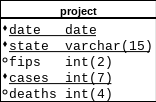
\includegraphics[scale=.95]{erdiagram.png} \\
Underlined values are primary keys, these make up a composite primary key \\
Hollow symbols (Circles) are allowed to be NULL \\
Solid symbols (Diamonds) are not allowed to be NULL

\end{document}

